%!TEX root = ../main.tex 

\section{Comment protéger une alimentation?}

\subsection{Protection antistatique}

\begin{frame}{Décharge Électrostatique (ESD)}
    \begin{columns}
        \begin{column}{0.66\textwidth}
            \begin{itemize}
                \item Norme IEC-61000-4-2
                \begin{itemize}
                    \item Types de décharges
                    \item Méthodologies de tests \& certification
                    \item 4 catégories de produits
                    \item Jusqu'à $\SI{\pm 8}{\kilo\volt}$ / $\SI{\pm 15}{\kilo\volt}$
                \end{itemize}
                \item Deux types de chocs statiques
                \begin{itemize}
                    \item \textbf{Contact Discharge} - Toucher directement chaque pin avec un ESD gun
                    \item \textbf{Air Discharge} - ESD gun proche du DUT jusqu'à décharge
                \end{itemize}
            \end{itemize}
        \end{column}

        \begin{column}{0.33\textwidth}
            \begin{figure}
                \centering
                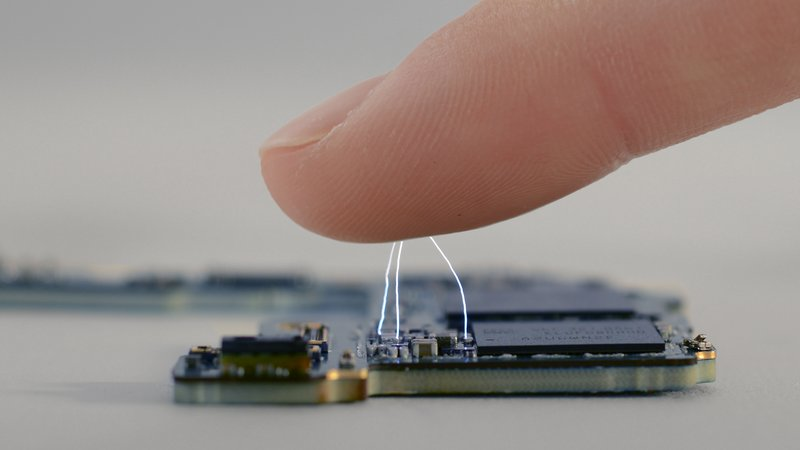
\includegraphics[width=\textwidth]{pictures/ESD-discharge-finger.png}
            \end{figure}
            \begin{figure}
                \centering
                
\includegraphics[width=0.5\textwidth]{pictures/ESD-logo.png}
            \end{figure}
        \end{column}
    \end{columns}
\end{frame}

\begin{frame}{Décharge Électrostatique - Waveform}
    \begin{columns}
        \begin{column}{0.6\textwidth}
        \end{column}
        \begin{column}{0.5\textwidth}
            \begin{itemize}
                \item Pic de courant initial
                \begin{itemize}
                    \item Rise time $\lesssim \SI{1}{\nano\second}$
                \end{itemize}
                \item $2^e$ pic
                \item Chute graduelle
            \end{itemize}
        \end{column}
    \end{columns}

    \vspace{-66pt}

    \begin{figure}
        \centering
        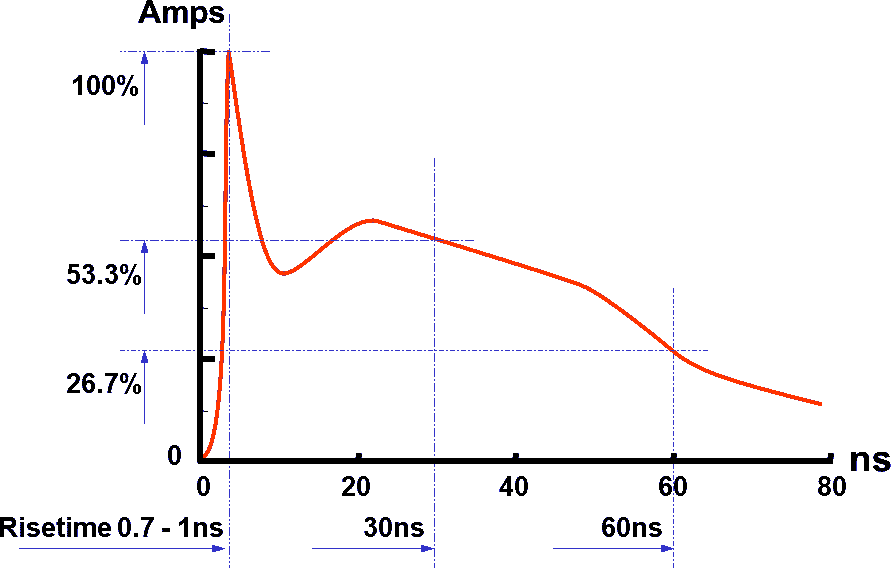
\includegraphics[width=\textwidth, height=0.8\textheight, keepaspectratio]{pictures/ESD-discharge-waveform.png}
    \end{figure}
\end{frame}

\begin{frame}{Circuit protégé antistatiquement - Zener}
    \begin{center}
    \vspace{-24pt}
    \resizebox{\textwidth}{0.8\textheight}{
    \begin{circuitikz}[american voltages]
        \draw [thick]
        (0,-3) to [short, *-] (10,-3)
        to [european resistor, l_=${LOAD}$] (10,1)
        (0,-3) to [open, v<=$V$] (0,1)
        to [short] (10,1)
        ;

        \draw [thick]
        (3, -3) to [empty ZZener diode, color=red] (3, 1);

        % Current spike as a waveform
        \draw[thick, ->] (-0.1, 2) -- (0,3) % Rising edge
        -- (0,3) -- (0.1,1.8) % First sharp drop
        -- (0.2,2.5) -- (0.3,1.9) % Second spike
        -- (0.4,2.3) -- (0.5,2.0) % Smaller oscillation
        -- (0.6,2.15) -- (0.7,2.05) % Final damping
        -- (1,2.1); % Settling

        \node[right] at (1,2.1) {$i_{\text{ESD}}(t) \rightarrow \SI{8}{\kilo\volt}$};
    \end{circuitikz}
    }
    \end{center}
\end{frame}

\begin{frame}{Diode Normale - IV Curve}
    \begin{figure}
        \centering
        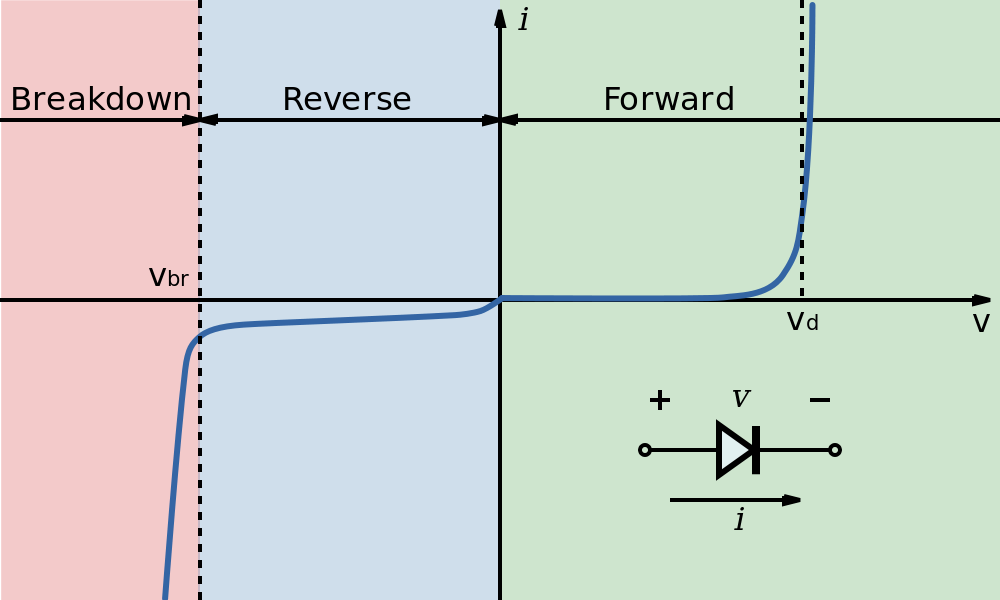
\includegraphics[width=\textwidth, height=0.8\textheight, keepaspectratio]{pictures/diode-iv-curve.png}
    \end{figure}
\end{frame}

\begin{frame}{Diode Zener}
    \begin{columns}
        \begin{column}{0.4\textwidth}
            \begin{itemize}
                \item \textbf{Faite pour être mise à l'envers!}
                \bigskip
                \item $V_Z$ contrôlé
                \item Beaucoup de courant en avalanche
                \item N'endommage pas la diode
                \bigskip
                \item Utilisé dans des références de tension
                \item Utilise comme protection antistatique
            \end{itemize}
        \end{column}
        \begin{column}{0.6\textwidth}
            \begin{figure}
                \centering
                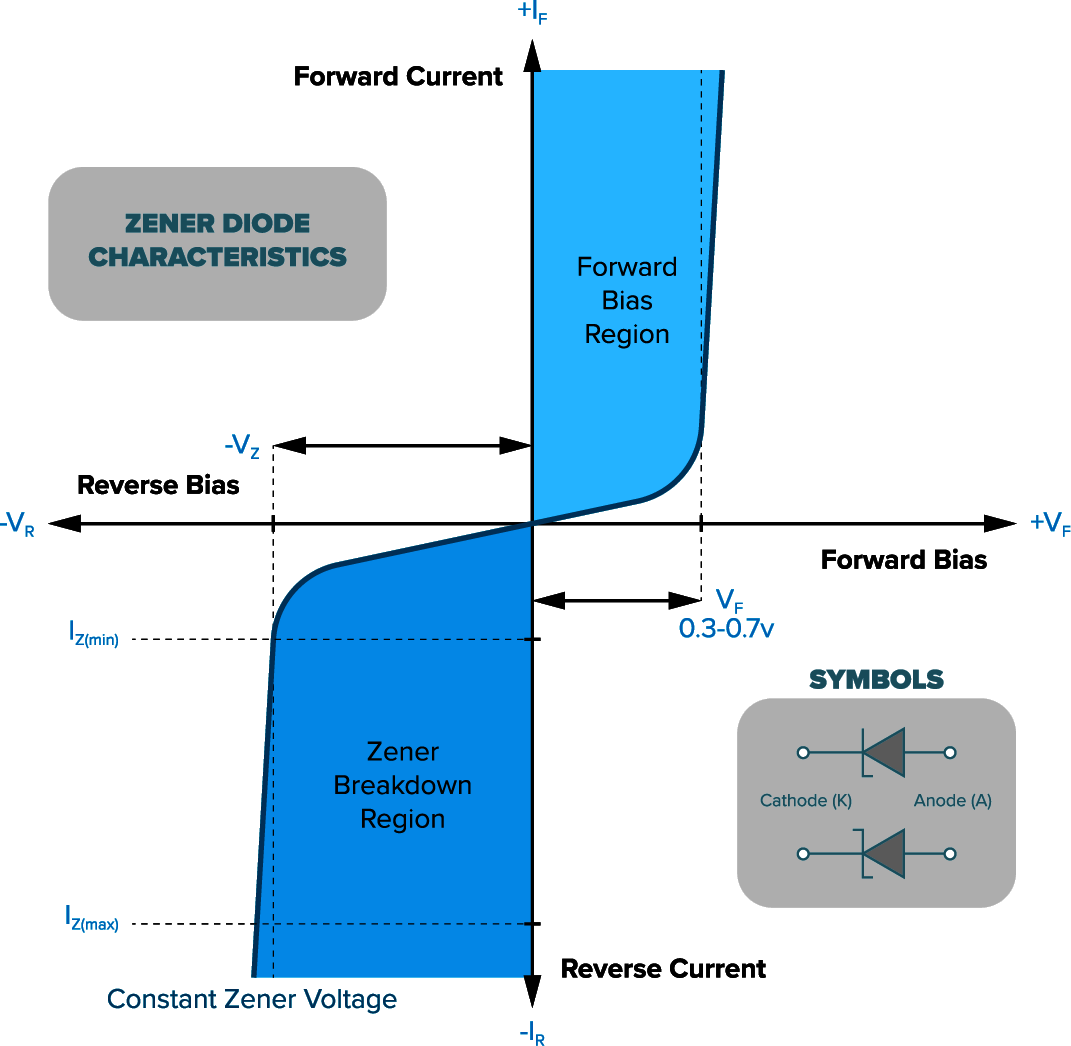
\includegraphics[width=\textwidth, height=0.8\textheight, keepaspectratio]{pictures/diode-zener-iv-curve.png}
            \end{figure}
        \end{column}
    \end{columns}
\end{frame}

\begin{frame}{Circuit protégé antistatiquement}
    \begin{center}
    \vspace{-24pt}
    \resizebox{\textwidth}{0.8\textheight}{
    \begin{circuitikz}[american voltages]
        \draw [thick]
        (0,-3) to [short, *-] (10,-3)
        to [european resistor, l_=${LOAD}$] (10,1)
        (0,-3) to [open, v<=$V$] (0,1)
        to [short] (10,1)
        ;

        \draw [thick]
        (3, -3) to [full ZZener diode, a=$\SI{15}{\volt}$] (3, 1);

        \draw[->, thick, red] 
        (1, 0.75) to[out=0, in=90] (2.75, -0.5);

        % Current spike as a waveform
        \draw[thick, ->]
           (-0.1, 2) -- (0,3)       % Rising edge
        -- (0,3) -- (0.1,1.8)       % First sharp drop
        -- (0.2,2.5) -- (0.3,1.9)   % Second spike
        -- (0.4,2.3) -- (0.5,2.0)   % Smaller oscillation
        -- (0.6,2.15) -- (0.7,2.05) % Final damping
        -- (1,2.1);                 % Settling

        \node[right] at (1,2.1) {$i_{\text{ESD}}(t) \rightarrow \SI{8}{\kilo\volt}$};
    \end{circuitikz}
    }
    \end{center}
\end{frame}


\begin{frame}{Protection avec une diode Zener}
    \begin{itemize}
        \item Clamp le pulse à $V_Z$
        \item Protège les dispositifs par apprès
        \bigskip
        \item Pas l'option la plus rapide
        \item Ne protège pas contre un pulse négatif 
    \end{itemize}

    \begin{figure}
        \centering
        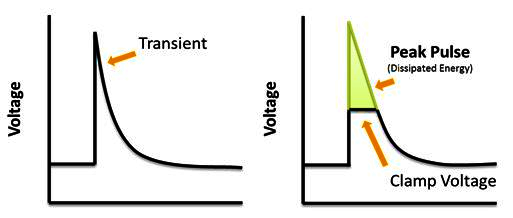
\includegraphics[width=\textwidth, height=0.5\textheight, keepaspectratio]{pictures/clamping-esd-pulse.png}
    \end{figure}
\end{frame}


\begin{frame}{Circuit protégé antistatiquement - TVS}
    \begin{center}
    \vspace{-24pt}
    \resizebox{\textwidth}{0.8\textheight}{
    \begin{circuitikz}[american voltages]
        \draw [thick]
        (0,-3) to [short, *-] (10,-3)
        to [european resistor, l_=${LOAD}$] (10,1)
        (0,-3) to [open, v<=$V$] (0,1)
        to [short] (10,1)
        ;

        \draw [thick]
        (3, -3) to [empty TVS diode, color=red] (3, 1);

        % Current spike as a waveform
        \draw[thick, ->] (-0.1, 2) -- (0,3) % Rising edge
        -- (0,3) -- (0.1,1.8) % First sharp drop
        -- (0.2,2.5) -- (0.3,1.9) % Second spike
        -- (0.4,2.3) -- (0.5,2.0) % Smaller oscillation
        -- (0.6,2.15) -- (0.7,2.05) % Final damping
        -- (1,2.1); % Settling

        \node[right] at (1,2.1) {$i_{\text{ESD}}(t) \rightarrow \pm\SI{8}{\kilo\volt}$};

        \draw[->, thick, red] 
        (1, 0.75) to[out=0, in=90] (2.75, -0.25);

        \draw[->, thick, blue] 
        (1, -2.75) to[out=0, in=-90] (2.75, -1.75);
    \end{circuitikz}
    }
    \end{center}
\end{frame}

\begin{frame}{Diode TVS (Transient Voltage Suppression)}
    \begin{columns}
        \begin{column}{0.5\textwidth}
            \begin{itemize}
                \item \textbf{Faite pour protection antistatique!}
                \item \textbf{Bidirectionnel!!}
            \end{itemize}
        \end{column}
        \begin{column}{0.5\textwidth}
            \begin{itemize}
                \item Deux diodes Zener qui se font face
                \item \textit{iv curve} symmétrique
            \end{itemize}
        \end{column}
    \end{columns}
    \begin{figure}
        \centering
        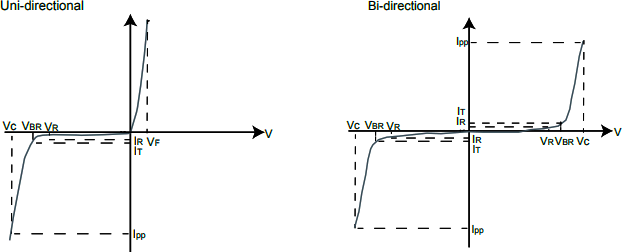
\includegraphics[width=\textwidth, height=0.55\textheight, keepaspectratio]{pictures/diode-tvs-iv-curve.png}
    \end{figure}
\end{frame}

\begin{frame}{Circuit protégé antistatiquement - Condensateur}
    \begin{center}
    \vspace{-24pt}
    \resizebox{\textwidth}{0.8\textheight}{
    \begin{circuitikz}[american voltages]
        \draw [thick]
        (0,-3) to [short, *-] (10,-3)
        to [european resistor, l_=${LOAD}$] (10,1)
        (0,-3) to [open, v<=$V$] (0,1)
        to [short] (10,1)
        ;

        \draw [thick]
        (3, -3) to [C, color=red] (3, 1);

        % Current spike as a waveform
        \draw[thick, ->] (-0.1, 2) -- (0,3) % Rising edge
        -- (0,3) -- (0.1,1.8) % First sharp drop
        -- (0.2,2.5) -- (0.3,1.9) % Second spike
        -- (0.4,2.3) -- (0.5,2.0) % Smaller oscillation
        -- (0.6,2.15) -- (0.7,2.05) % Final damping
        -- (1,2.1); % Settling

        \node[right] at (1,2.1) {$i_{\text{ESD}}(t) \rightarrow \pm\SI{8}{\kilo\volt}$};
    \end{circuitikz}
    }
    \end{center}
\end{frame}


\subsection{Protection de tension inverse}
\begin{frame}{Circuit de protection inverse - Diode}
    \begin{columns}
        \begin{column}{0.33\textwidth}
            \begin{itemize}
                \item Ne conduit que dans un sens
                \bigskip
                \item Drop de tension $V_f$
                \item $P = I \cdot V_f$
            \end{itemize}
        \end{column}
        \begin{column}{0.66\textwidth}
            \begin{center}
            \vspace{-24pt}
            \resizebox{\textwidth}{!}{
            \begin{circuitikz}[american voltages]
                \draw [thick]
                (0, 0) to [short, *-] (10, 0)
                to [european resistor, l_=${LOAD}$] (10, 5)
                (0, 0) to [open, v<=$V$] (0, 5)
                to [short] (4, 5)
                to [empty diode, color=red] (6, 5)
                to [short] (10, 5)
                ;
            \end{circuitikz}
            }
            \end{center}
        \end{column}
    \end{columns}
\end{frame}

\begin{frame}{Circuit de protection inverse - Diode Schottky}
    \begin{columns}
        \begin{column}{0.33\textwidth}
            \begin{itemize}
                \item Ne conduit que dans un sens
                \bigskip
                \item Drop de tension $V_f$ plus petite
                \item $P = I \cdot V_f$
                \bigskip
                \item Plus cher pour même rating de courant
            \end{itemize}
        \end{column}
        \begin{column}{0.66\textwidth}
            \begin{center}
            \vspace{-24pt}
            \resizebox{\textwidth}{!}{
            \begin{circuitikz}[american voltages]
                \draw [thick]
                (0, 0) to [short, *-] (10, 0)
                to [european resistor, l_=${LOAD}$] (10, 5)
                (0, 0) to [open, v<=$V$] (0, 5)
                to [short] (4, 5)
                to [empty Schottky diode, color=red] (6, 5)
                to [short] (10, 5)
                ;
            \end{circuitikz}
            }
            \end{center}
        \end{column}
    \end{columns}
\end{frame}

\begin{frame}{Circuit de protection inverse - PMOS}
    \begin{columns}
        \begin{column}{0.33\textwidth}
            \begin{itemize}
                \item Ne conduit que dans un sens
                \bigskip
                \item Drop de tension vraiment plus petite ($R_{ds_{on}} \cdot I$)
                \bigskip
                \item Tension maximale supportée
            \end{itemize}
        \end{column}
        \begin{column}{0.66\textwidth}
            \begin{center}
            \vspace{-24pt}
            \resizebox{\textwidth}{!}{
            \begin{circuitikz}[american voltages]
                \draw [thick]
                (0, 0) to [short, *-] (10, 0)
                to [european resistor, l_=${LOAD}$] (10, 5)
                (0, 0) to [open, v<=$V$] (0, 5);
                
                \draw   (4,5) node[pigfete, bodydiode, color=red, rotate=90, xscale=2, yscale=-2] (fet) {}
                (fet.G) node [anchor=south, xshift=8pt] {G}
                (fet.D) node [anchor=west, yshift=8pt] {D}
                (fet.S) node [anchor=east, yshift=8pt] {S}
                (fet.G) to [short, -*] (fet.G |- 0,0)
                (fet.D) to [short, -*] (0, 5)
                (fet.S) to (10, 5);
            \end{circuitikz}
            }
            \end{center}
        \end{column}
    \end{columns}
\end{frame}

\begin{frame}{Transistor MOSFET P-Channel (PMOS)}
    \begin{columns}
        \begin{column}{0.75\textwidth}
            \begin{center}
                $V_{gs}$ négatif!\\
                \vspace{6pt}
                $V_{gs} < -V_t$\\
                \vspace{8pt}
                Faire attention au $V_{gs_{max}}$
            \end{center}
            \vspace{24pt}

            \begin{columns}
                \begin{column}{0.5\textwidth}
                    %\textbf{Branchement normal}
                    \begin{itemize}
                        \item $V_G = \SI{0}{\volt}$
                        \item $V_{gs} = -VDD$
                        \item $-VDD < -V_t$
                        \item Conduit!
                    \end{itemize}
                \end{column}
                \begin{column}{0.5\textwidth}
                    %\textbf{Branchement inverse}
                    \begin{itemize}
                        \item $V_G = VDD$
                        \item $V_{gs} = \SI{0}{\volt}$
                        \item $\SI{0}{\volt} > -V_t$
                        \item Ne conduit pas
                    \end{itemize}
                \end{column}
            \end{columns}
        \end{column}

        \begin{column}{0.25\textwidth}
            \begin{center}
            \vspace{-24pt}
            \resizebox{!}{0.75\textheight}{
            \begin{circuitikz}[american voltages]
                
                \draw   (2,0) node[pigfete, bodydiode, xscale=1.5, yscale=1.5] (fet) {}
                (fet.G) node [anchor=east, yshift=8pt] {G}
                (fet.D) node [anchor=south, xshift=8pt, yshift=-4pt] {D}
                (fet.S) node [anchor=north, xshift=8pt, yshift=4pt] {S}
                (fet.G) to [short, -*] (fet.G |- 0, 0.4)
                (fet.D) to [short] (2, 2)
                ++(0,0) node[vcc]{VDD}
                (fet.S) to [short] (2, -1.5)
                to [R] (2, -3.5)
                to (2, -3.75) node[ground]{}
                ;

                \draw[->, thick, red] 
                (1, 0.75) to[out=90, in=180] (1.75, 1.5);

                \node[right] at (0.66, 1.66) {$V_{gs}$};
            \end{circuitikz}
            }
            \end{center}
        \end{column}
    \end{columns}
\end{frame}

\begin{frame}{Circuit de protection inverse - PMOS complèt}
    \begin{columns}
        \begin{column}{0.33\textwidth}
            \begin{itemize}
                \item Ne conduit que dans un sens
                \bigskip
                \item Drop de tension vraiment plus petite ($R_{ds_{on}} \cdot I$)
                \bigskip
                \item Supporte toutes les tensions!
            \end{itemize}
        \end{column}
        \begin{column}{0.66\textwidth}
            \begin{center}
            \vspace{-24pt}
            \resizebox{\textwidth}{!}{
            \begin{circuitikz}[american voltages]
                \draw [thick]
                (0, 0) to [short, *-] (10, 0)
                to [european resistor, l_=${LOAD}$] (10, 5)
                (0, 0) to [open, v<=$V$] (0, 5);
                
                \draw   (4,5) node[pigfete, bodydiode, rotate=90, xscale=2, yscale=-2] (fet) {}
                (fet.G) node [anchor=south, xshift=8pt] {G}
                (fet.D) node [anchor=west, yshift=8pt] {D}
                (fet.S) node [anchor=east, yshift=8pt] {S}
                (fet.G) to [R, -*] (fet.G |- 0, 0)
                (fet.D) to [short, -*] (0, 5)
                (fet.S) to (10, 5)
                (fet.G) to [short, *-] (fet.G -| 6,3)
                to [empty ZZener diode, color=red] (6, 5);
            \end{circuitikz}
            }
            \end{center}
        \end{column}
    \end{columns}
\end{frame}


\subsection{Protection de court-circuit}

\begin{frame}{Fusible}
    \begin{columns}
        \begin{column}{0.5\textwidth}
            \begin{itemize}
                \item Chauffage d'un filament central
                \item Coupe un circuit lorsque trop de courant passe
                \bigskip
                \item Usage unique
                \item Lent à agir
            \end{itemize}
            \vspace{12pt}
            \begin{figure}
                \centering
                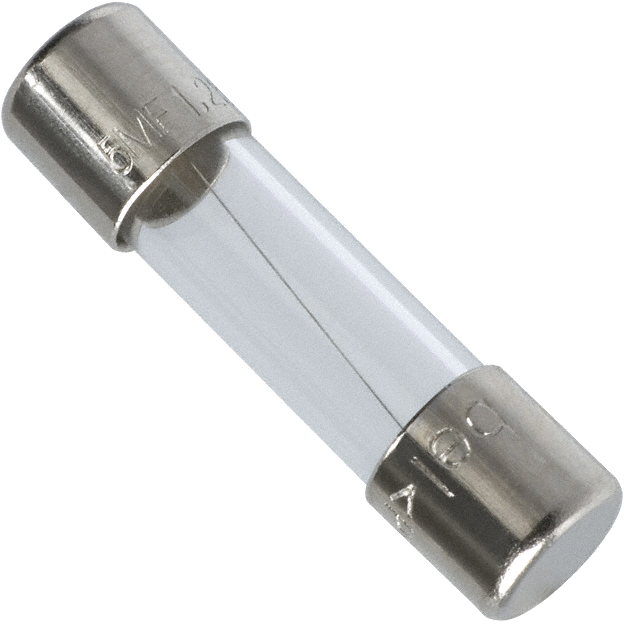
\includegraphics[width=0.33\textwidth]{pictures/fuse.png}
            \end{figure}
        \end{column}

        \begin{column}{0.6\textwidth}
            \vspace{-12pt}
            \begin{figure}
                \centering
                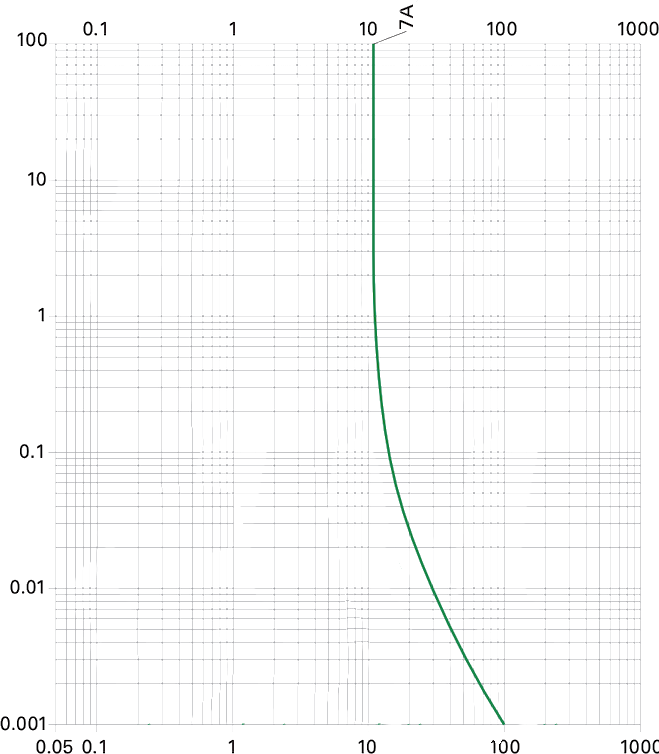
\includegraphics[width=\textwidth, height=0.75\textheight, keepaspectratio]{pictures/fuse-curve.png}
            \end{figure}
        \end{column}
    \end{columns}
\end{frame}

\begin{frame}{Polyfuse - Polyswitch - PTC - Resettable Fuse}
    \begin{columns}
        \begin{column}{0.6\textwidth}
            \begin{itemize}
                \item \textit{Positive Temperature Coefficient}
                \item Augmente sa résistance alors qu'il chauffe
                \item Utilisé comme thermistor
                \bigskip
                \item Usage multiple
                \item Lent à agir
                \item Prend du temps à se self-reset
            \end{itemize}
            \vspace{12pt}
            \begin{figure}
                \centering
                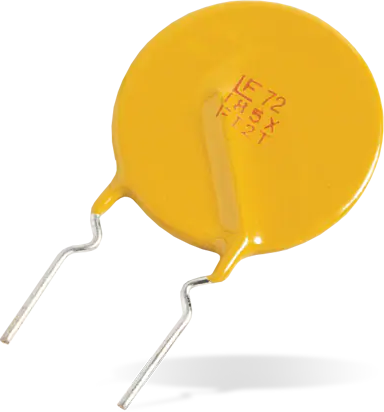
\includegraphics[width=0.25\textwidth]{pictures/polyfuse.png}
            \end{figure}
        \end{column}

        \begin{column}{0.4\textwidth}
            \begin{figure}
                \centering
                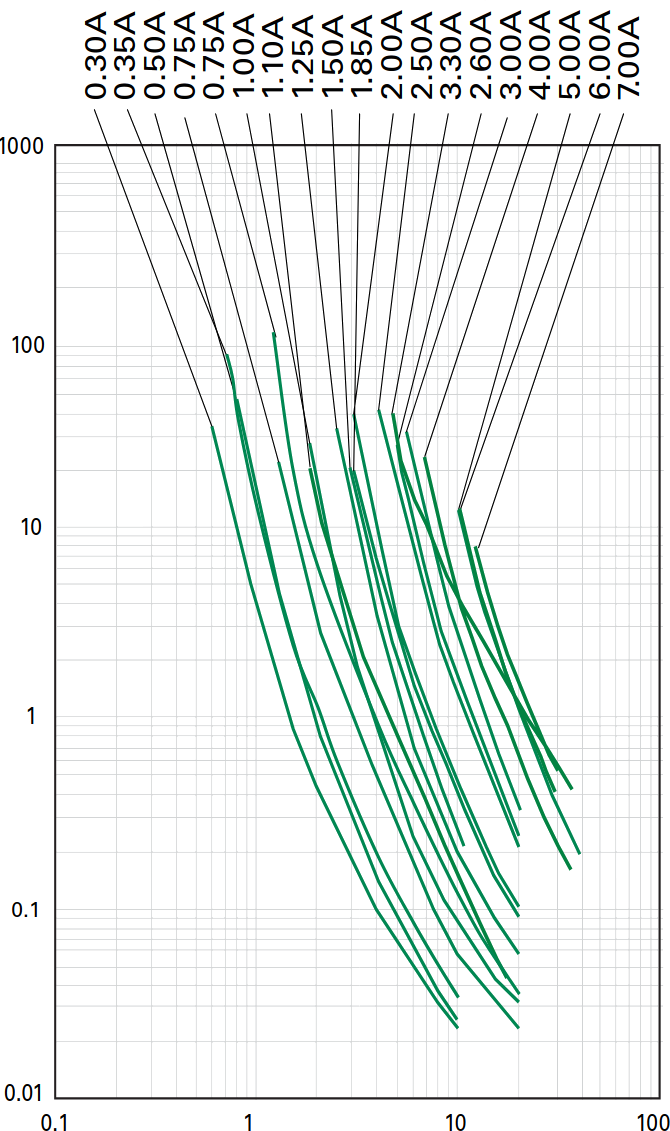
\includegraphics[width=\textwidth, height=0.75\textheight, keepaspectratio]{pictures/polyfuse-curve.png}
            \end{figure}
        \end{column}
    \end{columns}
\end{frame}

\subsection{Protection de inrush current}

\begin{frame}{Inrush Current}
    \begin{itemize}
        \item Tous les condensateurs d'un circuit sont des court-circuits
        \item Courant qui dépasse les spécifications pour charger les condensateurs
        \bigskip
        \item<2-> Spécification USB 2.0: $\SI{10}{\micro\farad}$
    \end{itemize}

    \vfill
    \begin{figure}
        \centering
        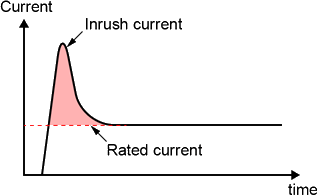
\includegraphics[height=0.55\textheight]{pictures/inrush-current.png}
    \end{figure}
\end{frame}

\begin{frame}{Inrush Current Limiter}
    \begin{columns}
        \begin{column}{0.6\textwidth}
            \textbf{Comment limiter la surge initiale?}
            \vspace{12pt}
            \begin{itemize}
                \item<1-> NTP
                \begin{itemize}
                    \item<1-> \textit{Negative Temperature Coefficient}
                    \item<1-> Conduit de plus en plus alors qu'il chauffe!
                \end{itemize}
                \bigskip
                \item<2-> Circuit de MOSFET
                \begin{itemize}
                    \item<2-> Charge d'un condensateur à la gate
                    \item<2-> Laisse passer de plus en plus de courant
                \end{itemize}
                \bigskip
                \item<3-> \textit{Soft-Start}
                \item<3-> \textit{Pre-Charge}
            \end{itemize}
        \end{column}

        \begin{column}{0.4\textwidth}
            \begin{figure}
                \centering
                \includegraphics<1->[width=0.4\textwidth]{pictures/inrush-current-limiter.png}
            \end{figure}
            \begin{figure}
                \centering
                \includegraphics<2->[width=\textwidth]{pictures/inrush-current-limiter-pmos.png}
            \end{figure}
        \end{column}
    \end{columns}
\end{frame}

\begin{frame}{Soft Start}
    \begin{columns}
        \begin{column}{0.575\textwidth}    
            \begin{itemize}
                \item Fonctionalité de certains régulateurs de tension
                \item Pente de la tension de sortie
                \item Ajustée avec un condensateur $C_{SS}$
            \end{itemize}
        \end{column}
        \begin{column}{0.4\textwidth}
            \begin{figure}
                \centering
                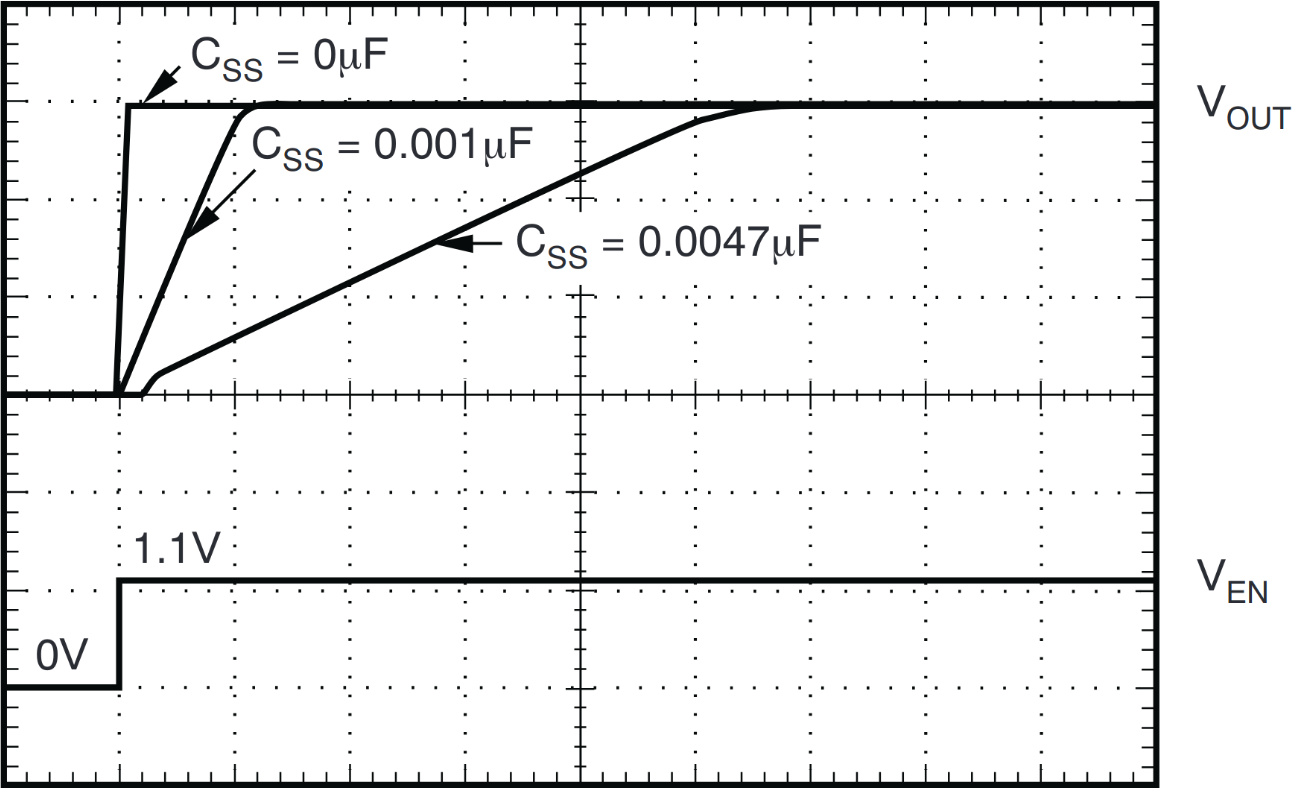
\includegraphics[width=0.9\textwidth]{pictures/ic-soft-start-curve.png}
            \end{figure}
        \end{column}
    \end{columns}
    \vfill
    \begin{figure}
        \centering
        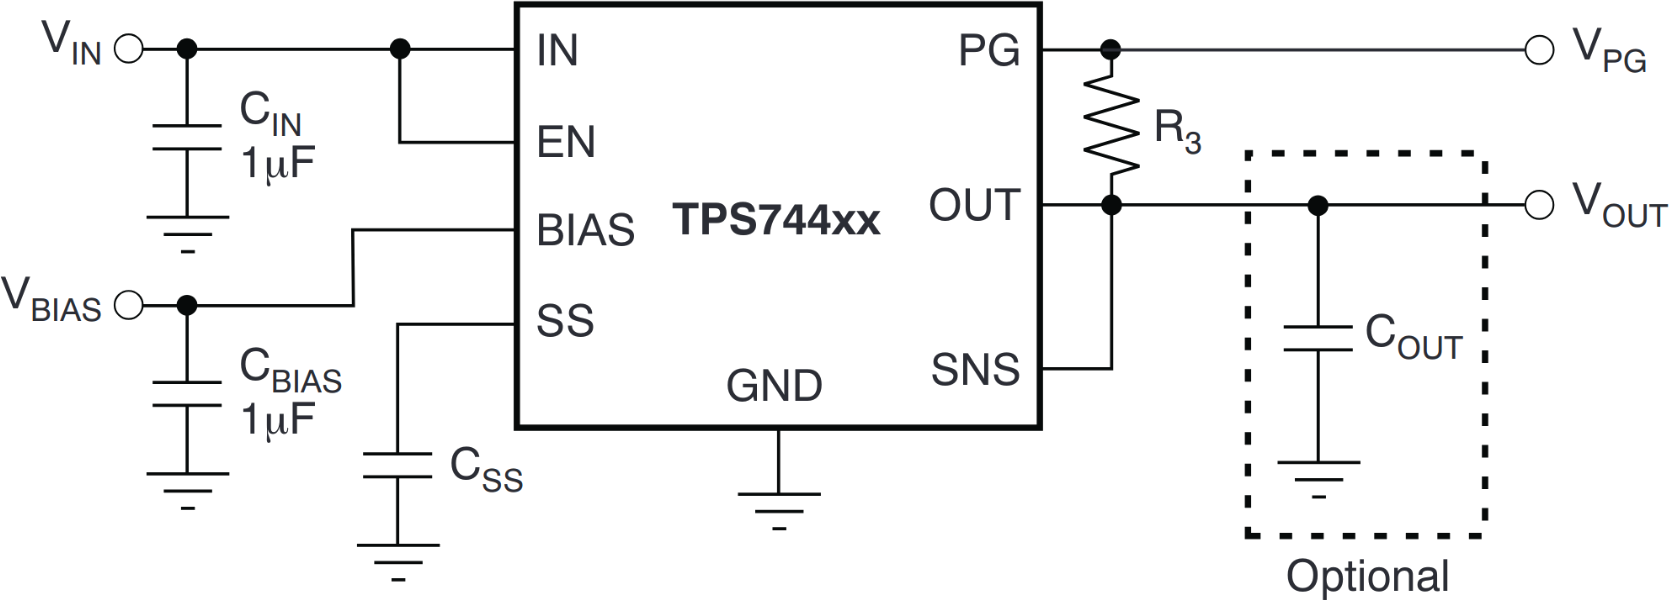
\includegraphics[width=0.66\textwidth]{pictures/ic-soft-start.png}
    \end{figure}
\end{frame}

\begin{frame}{Pre-charge}
    \begin{itemize}
        \item Pour les systèmes haut-voltage
        \item Contacteur avec une limite de courant
        \item Permet de charger les condensateurs
        \item Activation du contacteur principal après
    \end{itemize}

    \vfill

    \begin{center}
        \resizebox{!}{0.5\textheight}{
        \begin{circuitikz}[american voltages]
            \draw [thick]
            (0, 0) to [short, *-] (10, 0)
            to [european resistor, l_=${LOAD}$] (10, 5)
            (8, 5) to [short, *-] (8, 4) 
            to [C, color=red] (8, 1)
            to [short, -*] (8,0)
            (0, 0) to [open, v<=$400V$] (0, 5)
            to [short] (3, 5)
            to [normal open switch] (5, 5)
            to [short] (10, 5)
            (2, 5) to [short, *-] (2, 3)
            to [closing switch, color=red] (4, 3)
            to [R] (6, 3)
            to [short, -*] (6, 5)
            ;
        \end{circuitikz}
        }
    \end{center}    
\end{frame}

\subsection{Undervoltage Lockout}

\begin{frame}{Undervoltage Lockout (UVLO)}
\large
\centering
\begin{tabular}{c l}
    \textcolor{UDSgreenFierte}{\faPowerOff}       & Couper l'alimentation si entrée trop faible \\
    \textcolor{UDSgreenFierte}{\faBatteryQuarter} & Protection de batterie \\
    \textcolor{UDSgreenFierte}{\faPercent}        & Efficacité \\
    \textcolor{UDSgreenFierte}{\faCheckCircle}    & Garantie de fonctionnement \\
    \textcolor{UDSgreenFierte}{\faBolt}           & Du OVP (\textit{Overvoltage Protection}) ça existe aussi \\
\end{tabular}

\vfill
\begin{figure}
    \centering
    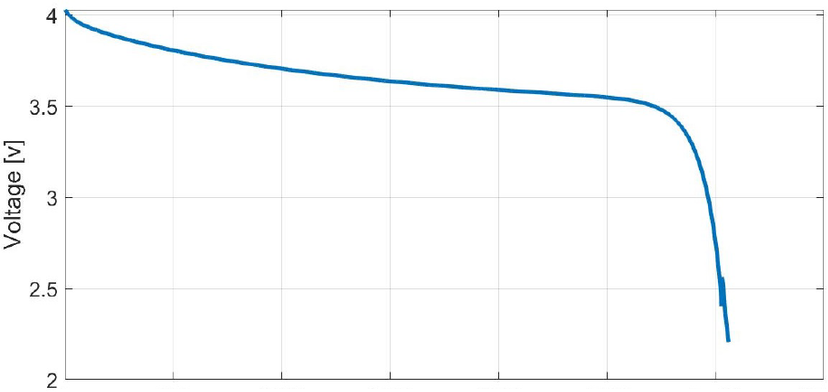
\includegraphics[width=0.66\textwidth, height=0.45\textheight, keepaspectratio]{pictures/battery-discharge-curve.png}
\end{figure}
\end{frame}

\begin{frame}{Undervoltage Lockout (UVLO) - Enable}
    \begin{columns}
        \begin{column}{0.66\textwidth}
            \begin{itemize}
                \item Batterie $V_{max} = \SI{4.2}{\volt}$
                \item Batterie $V_{min} = \SI{3.7}{\volt}$
                \item Tension EN $V_{ref} = \SI{1.2}{\volt}$
            \end{itemize}
        \end{column}

        \begin{column}{0.33\textwidth}
        \begin{center}
            Poser $R_2 = \SI{47}{\kilo\ohm}$\\
            \vspace{8pt}
            $V_{ref} = V_{min} \cdot \dfrac{R_2}{R_1 + R_2}$\\
            \vspace{6pt}
            $R_1 = $\SI{100}{\kilo\ohm}
        \end{center}
        \end{column}
    \end{columns}

    \vfill

    \begin{center}
        \resizebox{!}{0.5\textheight}{
        \begin{circuitikz}[american voltages]
        \ctikzset{multipoles/thickness=4}
        \ctikzset{multipoles/external pins thickness=2}
            % Regulator
            \draw (6, 5) node[dipchip,
                num pins=4,
                hide numbers,
                external pins width=0.3,
                external pad fraction=4 ](C){REG};
            \node [right, font=\tiny] at (C.bpin 1) {IN};
            \node [right, font=\tiny] at (C.bpin 2) {EN};
            \node [left,  font=\tiny] at (C.bpin 4) {OUT};

            % UVLO
            \draw (C.pin 2) to [short] (C.pin 2 -| 5, 5)
            to [R, l2=$R_1$ and $\SI{100}{\kilo\ohm}$, l2 halign=c] (C.pin 2 -| 2, 5) 
            to [short, -*] (C.pin 1 -| 2, 5)
            (C.pin 2 -| 5, 5) to [R, l2=$R_2$ and $\SI{47}{\kilo\ohm}$, l2 halign=c, -*] (5, 0);

            % Source & Load
            \draw
            (0, 0) to [short, *-] (10, 0)
            to [european resistor, l_=${LOAD}$] (C.pin 4 -| 10, 5)
            to [short] (C.pin 4)
            (C.pin 4 -| 9, 5) to [C, *-*] (9, 0)
            (0, 0) to [open, v<=$4.2V$] (C.pin 1 -| 0, 5)
            to [short] (C.pin 1);
        \end{circuitikz}
        }
    \end{center}  
\end{frame}


\subsection{Protection complète}

\begin{frame}{Protection complète - Circuit électrique}
    \begin{center}
        \resizebox{0.8\textwidth}{0.30\textheight}{
        \begin{tikzpicture}[
            block/.style = {rectangle, draw, minimum height=1cm,        minimum width=2.5cm, align=center},
            node distance=0.8cm and 0.6cm,
            >={Stealth[round]}
        ]
        
        % Nodes
\node[coordinate] (inlabel) {};
\node[block, right=of inlabel] (scp) {Short-circuit\\       Protection};
\node[block, right=of scp] (tvs) {Transient Voltage\\       Suppression};
\node[block, right=of tvs] (rvp) {Reverse Voltage\\     Protection};

\node[block, below=of scp] (uvlo) {Undervoltage\\Lockout};
\node[block, right=of uvlo] (ss) {Soft Start};
\node[block, right=of ss] (cm) {Current\\Measurement};
\node[coordinate, right=of cm] (outlabel) {};

% Input arrow with label
\draw[->] ($(inlabel)+(-0.75,0.0)$) -- (scp.west) node[     midway, above] {Input};

% Top row
\draw[->] (scp) -- (tvs);
\draw[->] (tvs) -- (rvp);

% Segmented down to second row
\draw[->] 
(rvp.east)      
-- ++(0.5, 0)     
-- ++(0, -0.85)    
-| (uvlo.north);


% Bottom row
\draw[->] (uvlo) -- (ss);
\draw[->] (ss) -- (cm);

% Output arrow with label
\draw[->] (cm.east) -- ++(1.25,0) node[midway, above] {Load};
        
        \end{tikzpicture}
        }
    \end{center}
    \pause
    \vspace{-12pt}
    \begin{center}
        \resizebox{\textwidth}{!}{
        \begin{circuitikz}[american voltages]
        \ctikzset{multipoles/thickness=4}
        \ctikzset{multipoles/external pins thickness=2}
            % Regulator
            \draw (18, 5) node[dipchip,
                num pins=6,
                hide numbers,
                external pins width=0.3,
                external pad fraction=4 ](C){REG};
            \node [right, font=\tiny] at (C.bpin 1) {IN};
            \node [right, font=\tiny] at (C.bpin 2) {EN};
            \node [right, font=\tiny] at (C.bpin 3) {SS};
            \node [left,  font=\tiny] at (C.bpin 6) {OUT};

            % Soft Start
            \draw
            (C.pin 3) to [short] (C.pin 3 -| 16, 5)
            to [C, l=$C_{SS}$, -*] (16, 0);

            % UVLO
            \draw (C.pin 2) to [short, -*] (C.pin 2 -| 15, 5)
            to [R] (C.pin 2 -| 13, 5) 
            to [short, -*] (C.pin 1 -| 13, 5)
            (C.pin 2 -| 15, 5) to [R, -*] (15, 0);

            % Source & Load
            \draw
            (0, 0) to [short, *-] (24, 0)
            to [european resistor, l_=${LOAD}$] (C.pin 6 -| 24, 5)
            to [R, l=$R_{CS}$] (C.pin 6)
            (C.pin 6 -| 23, 5) to [C, *-*] (23, 0)
            (0, 0) to [open, v<=$V$] (C.pin 1 -| 0, 5);

            % TVS
            \draw
            (C.pin 1 -| 4, 5) to [C, l_=$TVS$, *-*] (4, 0)
            (6, 0) to [full TVS diode, l_=$TVS$, *-*] (C.pin 1 -| 6, 5);

            % RVP
            \draw   (C.pin 1 -| 9, 5) node[pigfete, bodydiode, rotate=90, xscale=2, yscale=-2] (fet) {}
            (fet.G) node [anchor=south, xshift=8pt] {G}
            (fet.D) node [anchor=west, yshift=8pt] {D}
            (fet.S) node [anchor=east, yshift=8pt] {S}
            (fet.G) to [R, -*] (fet.G |- 0,0)
            %(fet.D) to [short, -*] (C.pin 1 -| 0, 5)
            (fet.S) to (C.pin 1)
            (fet.G) to [short, *-] (fet.G -| 11, 3)
            to [full ZZener diode, -*] (C.pin 1 -| 11, 5);

            % Fuse Protection
            \draw
            (C.pin 1 -| 0, 5) to [wfuse, l=$FUSE$] (C.pin 1 -| 4, 5)
            %to [R, l=$R_{CS}$] (C.pin 1 -| 4, 5)
            to [short] (fet.D);
            
        \end{circuitikz}
        }
    \end{center}  
\end{frame}

\begin{frame}{Solution Miracle}
    \vspace{-12pt}
    \begin{columns}
        \begin{column}{0.33\textwidth}
            \textbf<1>{Catégorie de device:}
            \begin{itemize}
                \item<1-> \textit{eFuse}
                \item<1-> \textit{Load Switch}
                \item<1-> \textit{Ideal Diode}
            \end{itemize}
        \end{column}
        \pause
        \begin{column}{0.66\textwidth}
            \begin{center}
                \textbf{Une seule chip qui:}
            \end{center}
            \begin{columns}
                \begin{column}{0.5\textwidth}
                    \begin{itemize}
                        \item \small{RVP}
                        \item \small{TVS}
                        \item \small{Short-Circuit}
                        \item \small{Current Limit}
                        \item \small{Current Monitoring}
                    \end{itemize}
                \end{column}
                \begin{column}{0.5\textwidth}
                    \begin{itemize}
                        \item \small{Soft-Start}
                        \item \small{UVLO / OVP}
                        \item \small{Très faibles pertes}
                        \item \small{Température}
                    \end{itemize}
                \end{column}
            \end{columns}
            
        \end{column}
    \end{columns}
    \vfill
    \begin{figure}
        \centering
        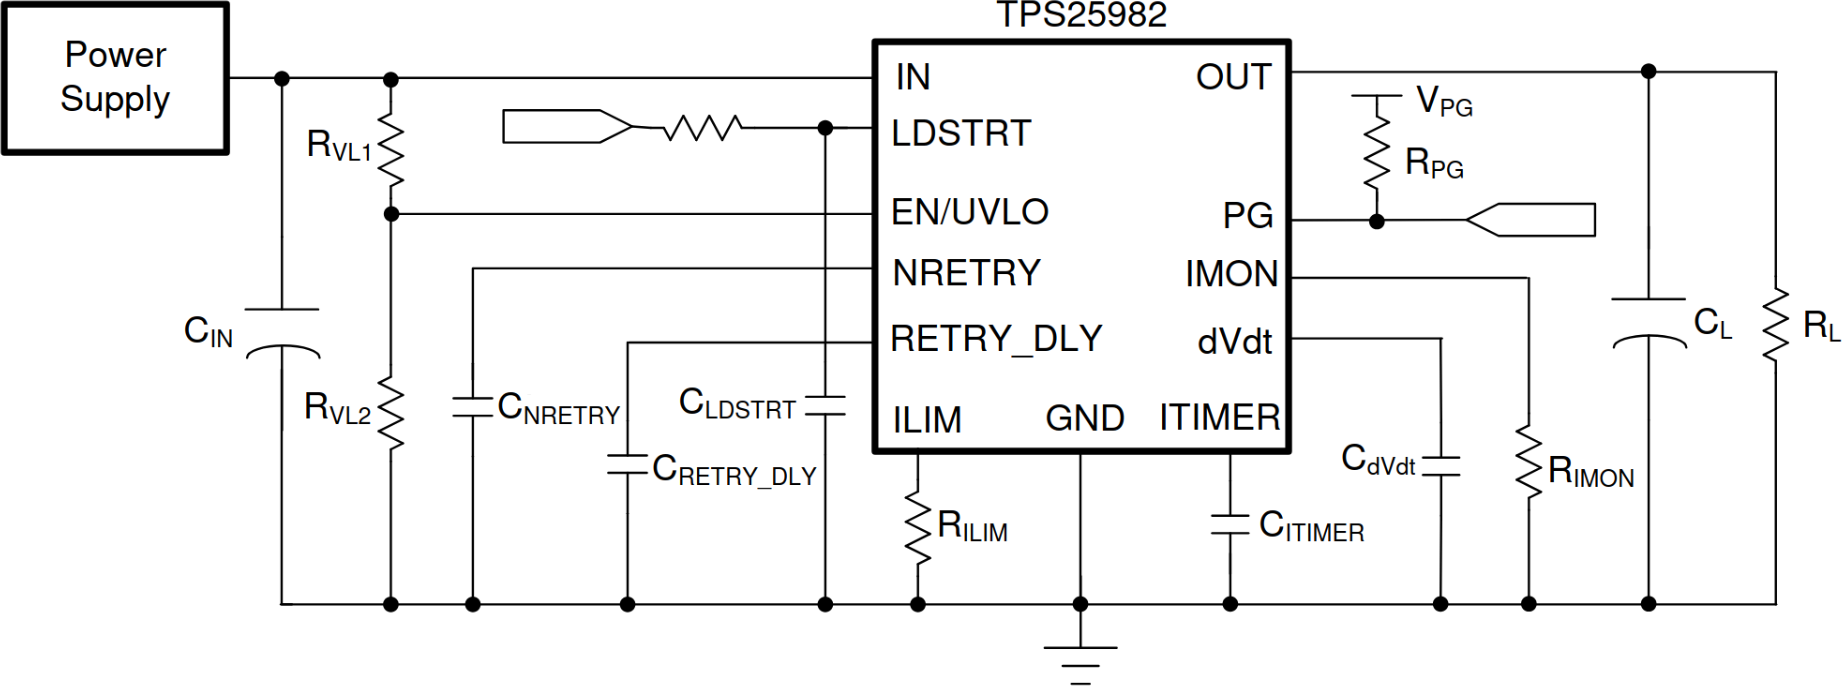
\includegraphics[width=0.75\textwidth, height=0.4\textheight, keepaspectratio]{pictures/load-switch.png}
    \end{figure}
\end{frame}


\subsection{120V}

\begin{frame}{120V}
    \begin{columns}
        \begin{column}{0.5\textwidth}
            \begin{itemize}
                \item<1-> Vivant (\textit{Live})
                \item<1-> Neutre (\textit{Neutral})
                \item<1-> Masse (\textit{Ground})
                \bigskip
                \item<2-> Pas le même GND que dans ton circuit
                \item<2-> GND du circuit provient du Neutre!
                \item<2-> \textbf{NE PAS CONNECTER ENSEMBLE}
            \end{itemize}
        \end{column}
        \begin{column}{0.5\textwidth}
            \begin{figure}
                \centering
                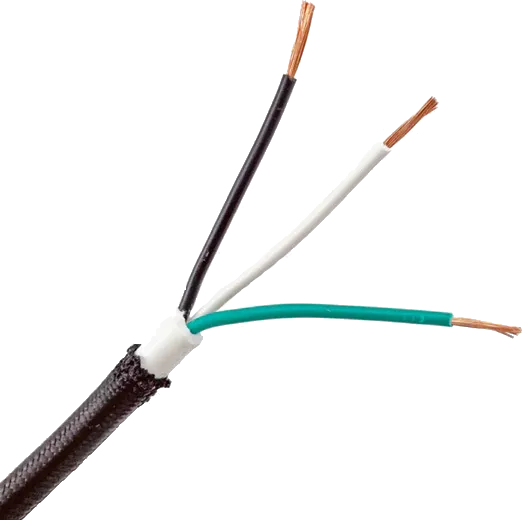
\includegraphics[width=0.75\textwidth]{pictures/120v-wire.png}
            \end{figure}
        \end{column}
    \end{columns}
\end{frame}

\begin{frame}{Connection 120V}
    \begin{center}
        \resizebox{\textwidth}{!}{
        \begin{circuitikz}[american]
            \ctikzset{voltage/american plus={\tiny $+$}};
            \ctikzset{voltage/american minus={\tiny $-$}};

            \draw (0,0) node [transformer](T){};

            \draw (T.A1) --++(-1,0);
            \draw (T.A2) --++(-1,0);
            \draw (T.B1) --++(3,0);        
            \draw (T.B2) --++(3,0);
            \draw (T.A2) to[open,v<=$\SI{25}{\kilo\volt}$](T.A1);

            \draw[thick]
            ($(T.B1)!0.5!(T.B2)-(0.7,0)$) --
            node[pos=0.25, above, inner sep=0pt](n){} ++
            (3,0);
            \draw  (n -| 2, 0) ++ (0, -0.03) -- ++ (0, -0.3) node[ground]{};

            \draw (n) to [open, v>={\footnotesize $\SI{120}{\volt}$}](T.B1);
            \draw (n) to [open, v>={\footnotesize $\SI{120}{\volt}$}](T.B2);
        \end{circuitikz}
        }
    \end{center}
\end{frame}

\begin{frame}{Grounding}
    \begin{itemize}
        \item Grounder les chassis des appareils
        \item Permet d'éviter d'avoir un chassis connecté au Live
        \item Retourne se connecter au panneau électrique
        \item Wiré séparément au Neutre
    \end{itemize}

    \vspace{-12pt}
    \begin{figure}
        \centering
        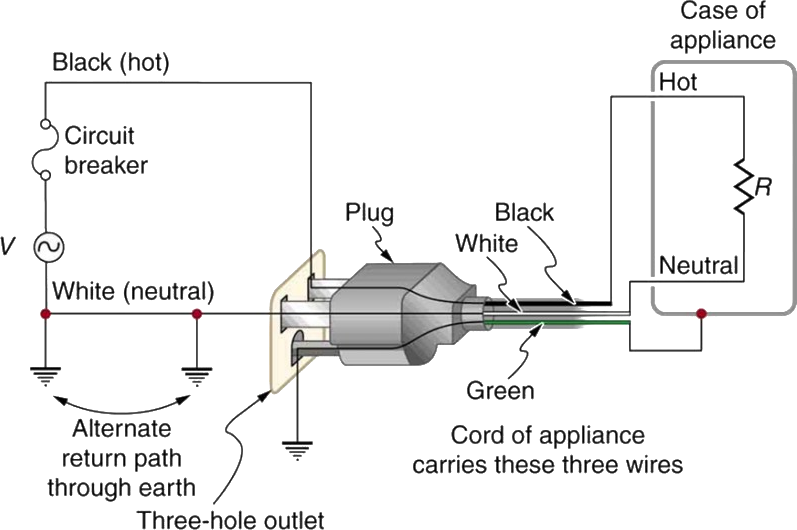
\includegraphics[width=0.66\textwidth, height=0.6\textheight, keepaspectratio]{pictures/3-wire-ac-plug.png}
    \end{figure}
\end{frame}

\begin{frame}{Grounding - Bonnes pratiques}
    \begin{columns}
        \begin{column}{0.6\textwidth}
            \begin{itemize}
                \item Garder le fil de GND plus long que les autres
                \item Mettre le LIVE plus court que les autres
                \item Toujours mettre du strain relief sur un câble
            \end{itemize}
            \vspace{-12pt}
            \begin{figure}
                \centering
                \includegraphics<1->[width=\textwidth, height=0.6\textheight, keepaspectratio]{pictures/uk-plug-wiring.png}
            \end{figure}
        \end{column}
        \begin{column}{0.4\textwidth}
            \begin{itemize}
                \item<2-> Grounder toutes les parties d'un boîtier
                \item<2-> Busbar de GND
            \end{itemize}
            \begin{figure}
                \centering
                \includegraphics<2->[width=\textwidth]{pictures/server-door-grounding.png}
            \end{figure}
        \end{column}
    \end{columns}
\end{frame}

\begin{frame}{Ground Fault Circuit Interrupter}
    \begin{columns}
        \begin{column}{0.7\textwidth}
            \begin{itemize}
                \item Mesure le courant qui passe par Live \& Neutral
                \item Coupe dès que $I_{in} \neq I_{out}$ 
            \end{itemize}
            \vspace{24pt}
            \begin{figure}
                \centering
                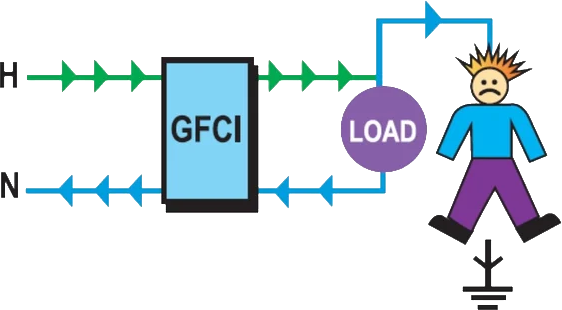
\includegraphics[width=0.75\textwidth]{pictures/gfci-example.png}
            \end{figure}
        \end{column}
        \begin{column}{0.3\textwidth}
            \begin{figure}
                \centering
                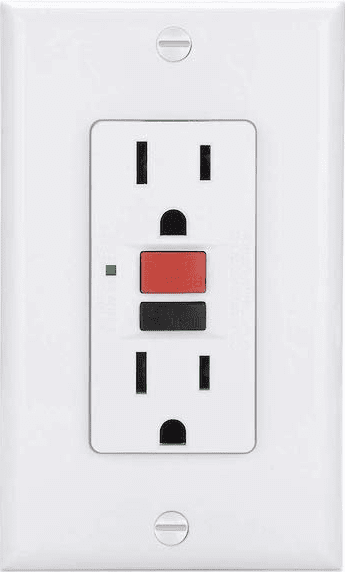
\includegraphics[width=0.6\textwidth]{pictures/gfci-outlet.png}
            \end{figure}
        \end{column}
    \end{columns}
\end{frame}